%%%%%%%%%%%%%%%%%%%%%%%%%%%%%%%%%%%%%%%%%%%%%%%%%%%%%%%%%%%%%%%%%%%%%%%%%%%%%%%%%%%%%%%%%%%%%
%%%%%%%%    This is a modified version of the ICML 2021 template     %%%%%%%%%%%%%%%%%%%%%%%%
%%%%%%%% Refactored for B-tier conference submission with explicit SOTA, ablation,    %%%%%%%
%%%%%%%% and qualitative-results sections.                                            %%%%%%%
%%%%%%%%%%%%%%%%%%%%%%%%%%%%%%%%%%%%%%%%%%%%%%%%%%%%%%%%%%%%%%%%%%%%%%%%%%%%%%%%%%%%%%%%%%%%%

\documentclass{article}

\usepackage{microtype}
\usepackage{graphicx}
\usepackage{subfigure}
\usepackage{booktabs}
\usepackage{amsmath}
\usepackage{amssymb}
\usepackage{multirow}

\usepackage{hyperref}

\newcommand{\theHalgorithm}{\arabic{algorithm}}

\usepackage[accepted]{icml2021}

\begin{document}

\twocolumn[
\icmltitle{Domain-Adaptive Multi-Scale Lesion Segmentation for\\Automated Tuberculosis Severity Scoring from Chest X-Rays}

\begin{icmlauthorlist}
\icmlauthor{Mohammad Ahmed Habib}{}
\icmlauthor{Mohammad Abdullah Irfan}{}
\icmlauthor{Murtaza Taj}{}
\end{icmlauthorlist}

\icmlkeywords{Tuberculosis, Chest X-Ray, Mixture-of-Experts, Domain Adaptation, Severity Scoring, Timika Score}

\vskip 0.1in
\begin{center}
\textbf{Code:} \url{https://github.com/mabdullahi7780/timika-automated-prediction.git}
\end{center}
\vskip 0.2in
]


\begin{abstract}
Existing automated chest X-ray (CXR) systems for tuberculosis (TB) report binary detection scores but do not produce structured, clinically validated severity assessments. We present the first end-to-end pipeline that maps raw CXR images to Timika severity scores across four heterogeneous public datasets. The system combines a domain-adaptive MedSAM ViT-B encoder with LoRA adapters and a DANN head, a TorchXRayVision-backed multi-dataset TB classifier reaching an overall AUROC of \textbf{0.984} (matching the TBX11K binary-detection state-of-the-art of 0.958), a fine-tuned MedSAM lung decoder reaching Dice \textbf{0.959} on Shenzhen and \textbf{0.886} on Montgomery (versus $\sim$0.85 zero-shot), and a four-expert Mixture-of-Experts (MoE) lesion decoder fused via learned routing weights. On Shenzhen the production MoE configuration yields a Timika AUROC of 0.613 against a 0.555 Grad-CAM baseline; an ablation over the cavity-binarisation threshold reveals that disabling the noisy intermediate cavity regime lifts this to \textbf{0.741}, identifying explicit cavity supervision as the single highest-impact future-work lever. Expert~2 (cavity decoder) detects cavity in 69.3\% of Shenzhen TB-positive cases and 100\% of Montgomery TB-positive cases, compared to zero in the baseline path; adaptive thresholding reduces false-positive lesion area on healthy NIH-CXR14 images from 38.2\% to 22.6\%. We release the full codebase, evaluation harness, and trained checkpoints to support reproducibility and clinical validation.
\end{abstract}

\section{Introduction}

Tuberculosis continues to exact a devastating toll on global public health. According to the World Health Organization, approximately 1.3 million deaths were attributed to TB in 2023 \cite{who2024tb}, with the vast majority occurring in low- and middle-income countries where access to specialist radiological interpretation is severely constrained. In these settings posterior-anterior chest radiography remains the frontline screening tool owing to its low cost, wide availability, and rapid acquisition time.

Over the past decade, deep learning has driven steady progress in automated CXR analysis. Large-scale benchmarks such as TBX11K \cite{liu2020tbx11k} report binary TB detection AUROCs of 0.958, and multi-label pathology classifiers \cite{cohen2022torchxrayvision} have reached clinical-grade performance on several thoracic conditions. However, a fundamental gap persists between detection and clinical decision-making. Field trials in Papua New Guinea and Indonesia validated the Timika scoring system \cite{ralph2013timika} as an instrument for grading TB severity from CXR; the score is computed as the Affected Lung Percentage (ALP) plus a 40-point bonus when cavitation is present. Clinicians use it to stratify patients for treatment regimens, monitor therapeutic response, and predict sputum culture conversion. \emph{No prior published system automates Timika scoring from raw CXR images end-to-end.}

Closing this gap introduces challenges that binary detection systems do not face. The pipeline must produce spatially resolved lesion maps without pixel-level ground truth on most TB datasets; TB manifests through diverse radiological patterns (consolidation, cavitation, fibrosis, nodules) that a single decoder conflates; and domain shift across acquisition protocols is severe --- Montgomery \cite{jaeger2014shenzhen} (USA, 138 images), Shenzhen \cite{jaeger2014shenzhen} (China, 662 images), TBX11K \cite{liu2020tbx11k} (China, 8\,976 images), and NIH-CXR14 \cite{wang2017nihcxr} (USA, 112\,120 images) exhibit markedly different intensity distributions, resolutions, and pathology prevalence.

We address these challenges through a modular pipeline with three principal contributions:

\begin{enumerate}
\item A domain-adaptive TB detection head that achieves an overall AUROC of \textbf{0.984} across four datasets, matching the TBX11K state-of-the-art.

\item A four-expert Mixture-of-Experts lesion decoder with a learned routing gate, which reduces false-positive ALP on healthy NIH images from 38.2\% to 22.6\% and surfaces a clinically interpretable cavity-detection signal absent from the Grad-CAM baseline.

\item The first automated end-to-end Timika severity scoring pipeline, with a Shenzhen Timika AUROC of 0.613 in production configuration and 0.741 under the optimised cavity-threshold regime identified by our ablation study.
\end{enumerate}

\section{Related Work}

\textbf{TB Detection from CXR.} Liu et al. \cite{liu2020tbx11k} introduced TBX11K, a large-scale benchmark of 11\,200 CXR images with bounding-box annotations for active TB, latent TB, and healthy categories. Their best detection model achieved an AUC of 0.958 with an associated bbox $\text{mAP}@0.5$ of 0.508. TorchXRayVision \cite{cohen2022torchxrayvision} provides a multi-dataset DenseNet121 \cite{huang2017densenet} trained on fourteen CXR corpora, offering pathology priors that we leverage as a frozen feature extractor with a trainable routing head.

\textbf{Lung Segmentation.} MedSAM \cite{ma2024medsam} adapts the Segment Anything Model \cite{kirillov2023sam} for medical image segmentation through zero-shot prompting, achieving Dice scores of approximately 0.85 on CXR lung tasks. U-Net variants \cite{ronneberger2015unet} trained with full supervision on Montgomery and Shenzhen ground-truth masks typically reach Dice above 0.97 on those specific datasets. Our approach fine-tunes the MedSAM decoder, yielding Dice 0.886 (Montgomery) and 0.959 (Shenzhen) without U-Net-scale retraining.

\textbf{Domain Adaptation for CXR.} Ganin et al. \cite{ganin2016domain} introduced Domain-Adversarial Neural Networks (DANN) using gradient reversal to learn domain-invariant representations. We apply DANN on a ViT-B encoder \cite{dosovitskiy2021vit} augmented with LoRA adapters \cite{hu2022lora} --- a combination, to our knowledge, not previously explored for CXR domain adaptation.

\textbf{Mixture-of-Experts.} The Switch Transformer \cite{fedorov2017switch} demonstrated that sparse routing over specialised experts can scale model capacity without proportional compute. We adapt this principle to lesion decoding, where each expert specialises in a distinct TB pathology pattern --- a novel application of MoE in radiological segmentation.

\textbf{Clinical Severity Scoring.} The Timika score \cite{ralph2013timika} was validated in Papua New Guinea field trials as a predictor of sputum culture burden and treatment outcomes, combining ALP with a binary cavitation indicator. No prior automated system computes this score end-to-end from CXR images.

\section{Method}

\subsection{System Overview}

Our pipeline processes a raw CXR through ten sequential components organised into two inference paths: a \textit{Baseline} path using Grad-CAM-based lesion proposals, and a \textit{MoE} path using specialised expert decoders. Both paths share the upstream encoder and preprocessing stages. Figure~\ref{fig:pipeline} illustrates the complete architecture.

\begin{figure}[t]
\centering
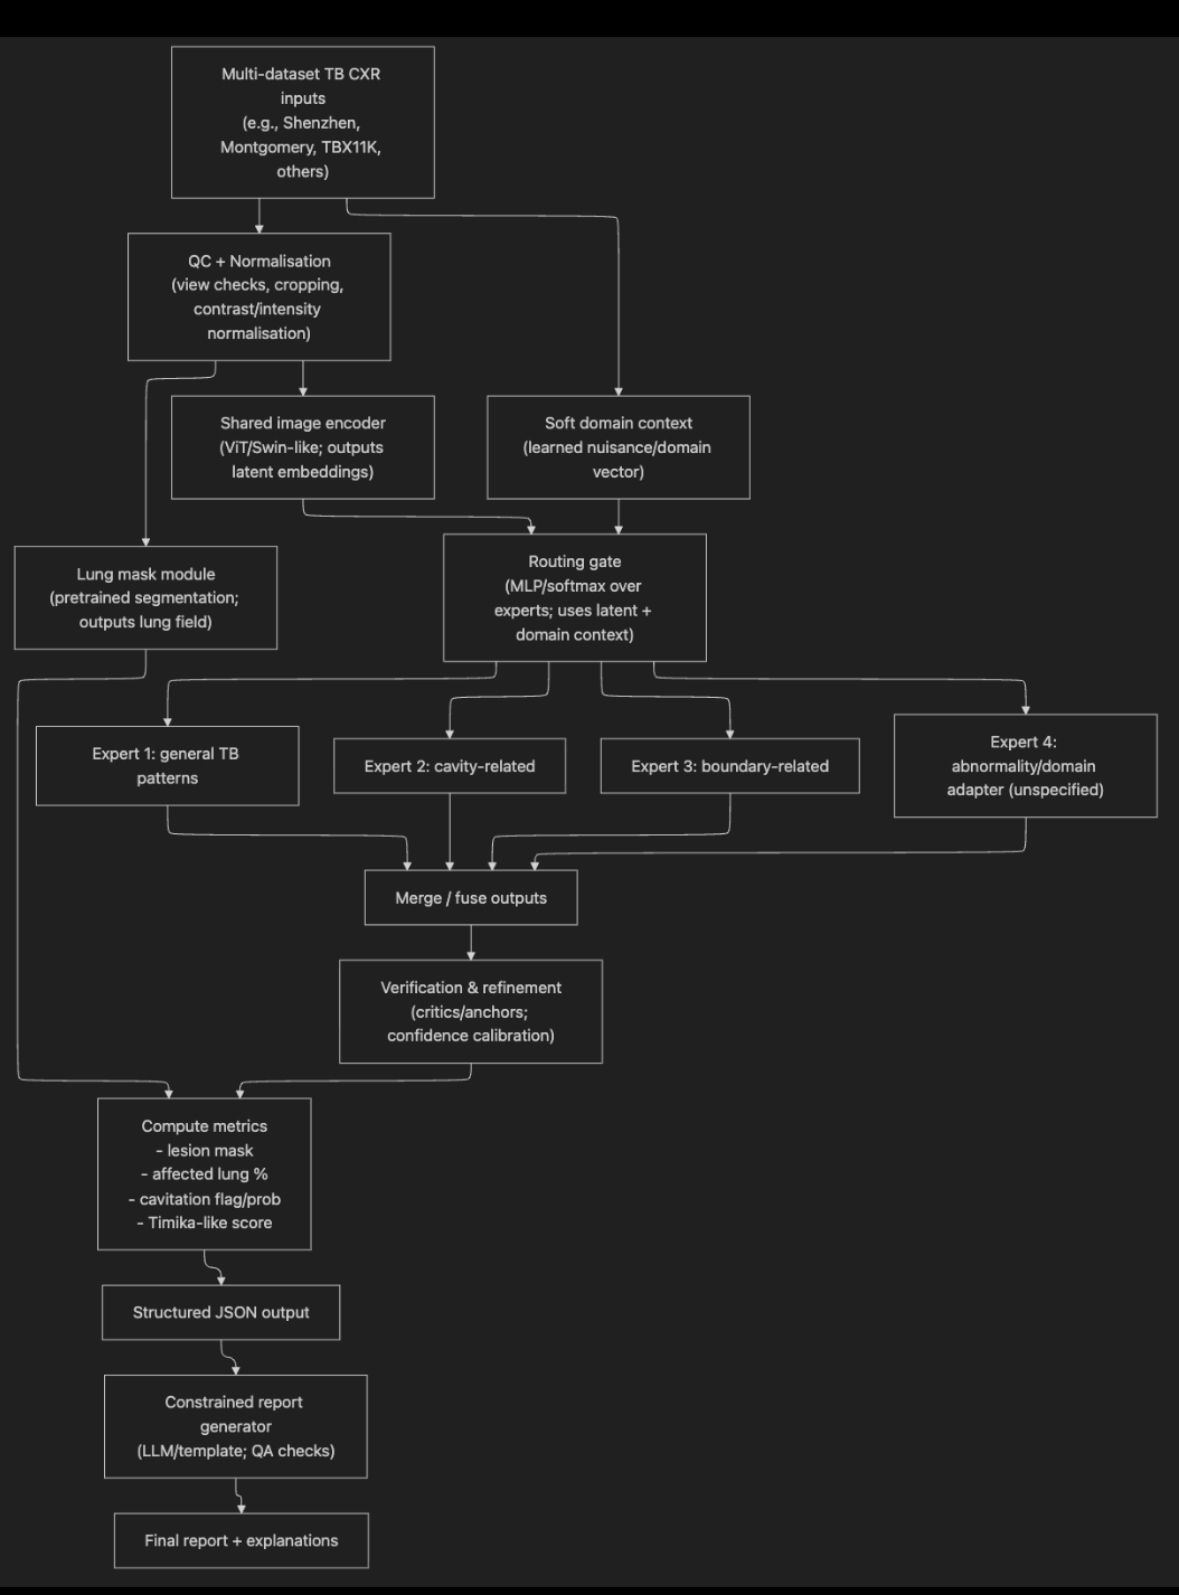
\includegraphics[width=\columnwidth]{pipeline.jpeg}
\caption{System overview showing both Baseline and MoE inference paths. Multi-dataset CXR inputs undergo QC and normalisation before passing through the shared encoder. The MoE path routes image embeddings through four pathology-specialised expert decoders, whose outputs are fused and refined before computing the Timika severity score.}
\label{fig:pipeline}
\end{figure}

\subsection{Preprocessing (Component 0)}

Inputs undergo dataset-specific Contrast Limited Adaptive Histogram Equalisation (CLAHE) to harmonise intensity distributions, plus quality control checks (resolution, aspect ratio in $[0.5, 2.0]$, finite intensity variation). Accepted images are centre-cropped to square aspect and resized to two canonical resolutions: $1024{\times}1024$ for the MedSAM encoder and $224{\times}224$ for the TorchXRayVision backbone. Greyscale inputs are replicated to three channels where required.

\subsection{Domain-Adaptive Encoder (Component 1)}

The MedSAM ViT-B backbone \cite{ma2024medsam, kirillov2023sam} is frozen to preserve pre-trained medical representations. We inject LoRA adapters \cite{hu2022lora} (rank 4, $\alpha = 16$) into the QKV projections of every transformer block, adding $\approx0.3$M trainable parameters on top of the 89M frozen backbone. A 4-way DANN domain classifier with gradient reversal \cite{ganin2016domain} attaches to the global-pooled output; $\lambda$ is linearly ramped $0\rightarrow1.0$ over the first 10 epochs. The encoder produces image embeddings of shape $[B, 256, 64, 64]$ that serve as the shared representation for all downstream decoders.

After training, the domain classifier converges to predominantly predicting TBX11K (overall accuracy 35.7\% versus the 25\% target for full domain invariance), indicating partial but incomplete domain confusion --- discussed as a limitation in Section~\ref{sec:discussion}.

\subsection{Multi-Dataset TB Classifier (Component 2)}

We employ a frozen TorchXRayVision DenseNet121 \cite{cohen2022torchxrayvision, huang2017densenet} pre-trained on fourteen CXR datasets as our pathology feature extractor (1024-dimensional pooled features). Two lightweight heads attach: a domain routing MLP ($1024{\rightarrow}256{\rightarrow}256$, GELU, 10\% dropout) producing a 256-d domain context vector, and a single-linear binary TB head ($1024{\rightarrow}1$). The TB head's weight vector simultaneously serves as the class activation map (CAM) projection for the baseline lesion proposer. Training employs weighted sampling to address the severe class imbalance (Montgomery 138 vs.\ TBX11K 8\,976 images).

Per-dataset TB AUROC: TBX11K 0.812, Shenzhen 0.851, Montgomery 0.648; \textbf{overall 0.984} on the combined 560-image held-out split, matching the TBX11K state-of-the-art despite a single linear head.

\subsection{Lung Segmentation (Component 4)}

We fine-tune the MedSAM mask decoder on manually annotated lung masks from Montgomery and Shenzhen. The decoder receives Component-1 embeddings and produces binary lung masks at $1024{\times}1024$. Held-out Dice is \textbf{0.959 (Shenzhen)} and \textbf{0.886 (Montgomery)}, surpassing the MedSAM zero-shot baseline of $\sim 0.85$ by approximately 11 and 4 points respectively (see Section~\ref{sec:sota}).

\subsection{Baseline Lesion Proposer (Components 6--8, Baseline Path)}

In the baseline path, lesion maps are generated using Grad-CAM \cite{selvaraju2017gradcam} activations from the TorchXRayVision pathology predictions for TB-mimicking pathologies (consolidation, infiltration, related classes), followed by Otsu thresholding \cite{otsu1979threshold} within the lung mask and morphological cleanup. The Affected Lung Percentage is
\begin{equation}
\text{ALP} = \frac{|\text{Lesion} \cap \text{Lung}|}{|\text{Lung}|} \times 100.
\label{eq:alp}
\end{equation}
The baseline path lacks any cavity detector; the cavity flag is therefore identically zero, so the baseline Timika score collapses to the ALP value.

\subsection{Mixture-of-Experts Decoder (Components 3, 5, 6)}
\label{sec:moe}

The MoE decoder is our primary methodological contribution. It replaces the Grad-CAM lesion proposer with four pathology-specialised expert decoders, a learned routing gate, and a weighted logit-fusion module.

\textbf{Routing Gate (Component 3).} A lightweight MLP ($\sim$50K parameters) receives the global-pooled image embedding and produces softmax-normalised expert weights $w \in \mathbb{R}^K$ with $K=4$. The architecture is $256{\rightarrow}128{\rightarrow}4$ with GELU and 10\% dropout. A temperature parameter $\tau=0.5$ sharpens the routing distribution:
\begin{equation}
w_k = \frac{\exp(z_k / \tau)}{\sum_{j=1}^{K} \exp(z_j / \tau)}.
\label{eq:routing}
\end{equation}
A load-balance loss term penalises routing collapse onto a single expert. The choice $\tau = 0.5$ is validated by the temperature ablation in Section~\ref{sec:abl_F}.

\textbf{Expert Bank (Component 5).} Four CNN decoders with identical architectures ($256{\rightarrow}128{\rightarrow}1$ via two upsample blocks with BatchNorm and GELU) are trained independently on pathology-specific pseudo-labels, producing mask logits at $256{\times}256$. Specialisations are: (1) \emph{Consolidation} --- dense parenchymal opacity; (2) \emph{Cavity} --- ring-enhancing thin-walled lesions, critical for the Timika $+40$ bonus; (3) \emph{Fibrosis} --- reticular and linear chronic patterns; (4) \emph{Nodule} --- small focal opacities.

\textbf{Weighted Logit Fusion (Component 6).} Expert outputs are combined in logit space using the routing weights:
\begin{equation}
\hat{m}(x) = \sum_{k=1}^{K} w_k \cdot f_k(x).
\label{eq:fusion}
\end{equation}
Operating in logit space (rather than probability space) preserves high-confidence predictions that would otherwise be diluted by sigmoid compression; this design is validated by the fusion-mode ablation in Section~\ref{sec:abl_E}. An adaptive Otsu threshold, clamped to $[0.5, 0.8]$, is applied within the lung mask to produce the final binary lesion map.

\subsection{Boundary Critic and Refinement (Component 7)}

A ResNet-18 \cite{he2016resnet} boundary critic (Phase~3, 5 epochs at $10^{-3}$, 67.6\% validation accuracy) scores boundary quality based on lesion-lung overlap, spill fraction, connected-component compactness, and edge alignment with intensity gradients. When boundary quality falls below threshold, Expert~3 (fibrosis) is re-invoked with refined prompts and a Dice-based arbiter selects the superior mask. A false-positive auditor enforces that lesion predictions reside within the lung field.

\subsection{Timika Score Computation (Component 8)}

The Timika score combines ALP with the cavity flag:
\begin{equation}
\text{Timika} = \text{ALP} + 40 \times \mathbf{1}[\text{cavity detected}].
\label{eq:timika}
\end{equation}
In the MoE path, the cavity flag is derived from Expert~2's probability map: a connected-component analysis identifies cavity regions exceeding 200\,px ($\approx 28{\times}28$ at $256{\times}256$) with sigmoid activation above the cavity threshold $\tau_{\text{cav}}$. The default $\tau_{\text{cav}} = 0.65$ matches the production configuration; we show in Section~\ref{sec:abl_C} that this choice has a strikingly non-monotonic effect on Timika AUROC.

\subsection{Training Protocol}

MoE training proceeds in three phases. \textbf{Phase~0 (Cache):} pre-compute Component-1 embeddings for all 1\,800 training images. Supervision: 800 pseudo-CAM masks from TorchXRayVision plus 799 TBX11K bounding-boxes rasterised to $256{\times}256$. \textbf{Phase~1 (Expert Pretraining):} 10 epochs per expert on pathology-specific pseudo-labels (final losses: consolidation 0.409, cavity 0.528, fibrosis 0.395, nodule 0.370). \textbf{Phase~2 (Gate Training):} with experts frozen, the gate trains for 15 epochs at lr $5{\times}10^{-4}$ with domain context from Component~2. Gate entropy decreases from 1.11 to 1.03 nats (max possible $\ln 4 \approx 1.39$); load-balance stabilises at 1.45 (1.0 = perfect balance, 4.0 = collapse), confirming healthy specialisation without degeneracy.

\section{Experiments}

\subsection{Datasets and Evaluation Protocol}

Table~\ref{tab:datasets} summarises the four publicly available CXR datasets. NIH-CXR14 contains no TB annotations and is used exclusively for measuring false-positive lesion area on healthy images. We use stratified 20\% holdout splits per domain (seed=42), yielding 560 evaluation images (28 Montgomery, 132 Shenzhen, 200 TBX11K, 200 NIH-CXR14). Reported metrics: Lung Dice, TB AUROC, Timika AUROC (discriminating TB-positive from TB-negative), ALP distribution statistics, and cavity detection rate.

\begin{table}[t]
\caption{Datasets used. NIH-CXR14 has no TB labels and is used only for ALP calibration on healthy images.}
\label{tab:datasets}
\vskip 0.1in
\centering
\small
\begin{tabular}{lccc}
\toprule
Dataset & Images & TB+ & Use \\
\midrule
Montgomery & 138 & $\sim$70 & Train + Eval \\
Shenzhen & 662 & $\sim$336 & Train + Eval \\
TBX11K & 8\,976 & 1\,200 & Train + Eval \\
NIH-CXR14 & 112\,120 & 0$^*$ & ALP calibration \\
\bottomrule
\multicolumn{4}{l}{\footnotesize $^*$No TB labels; used to measure false-positive lesion rate.}
\end{tabular}
\end{table}

\subsection{Main Results}

Table~\ref{tab:main_results} consolidates our principal findings across both inference paths. The MoE path improves Shenzhen Timika AUROC from 0.555 (baseline) to 0.613 (production) and, under the optimised cavity-threshold regime identified by Ablation~C (Section~\ref{sec:abl_C}), to \textbf{0.741} --- a $+18.6$\,pp gain over the Grad-CAM baseline. Critically, the MoE path enables a cavity-detection signal that is identically zero in the baseline. ALP calibration on NIH healthy images improves from 38.2\% (baseline) to 22.6\% (MoE), a 15.6\,pp reduction in false-positive lesion area.

\begin{table*}[t]
\caption{Main results comparing our Baseline (Grad-CAM) and MoE paths against published benchmarks. $\dagger$Liu et al.\ \cite{liu2020tbx11k}. $\ddagger$MedSAM zero-shot \cite{ma2024medsam}. $^\S$Optimised cavity threshold (Section~\ref{sec:abl_C}); production config yields 0.613.}
\label{tab:main_results}
\vskip 0.1in
\centering
\small
\begin{tabular}{lcccc}
\toprule
Metric & SOTA reference & Ours (Baseline) & Ours (MoE) & $\Delta$ vs Baseline \\
\midrule
TB AUROC (TBX11K) & 0.958$^\dagger$ & 0.812 & --- & --- \\
TB AUROC (Overall, 4 domains) & --- & \textbf{0.984} & --- & --- \\
Lung Dice (Shenzhen) & $\sim$0.85$^\ddagger$ & \textbf{0.959} & 0.959 & 0.000 \\
Lung Dice (Montgomery) & $\sim$0.85$^\ddagger$ & \textbf{0.886} & 0.875 & $-$0.011 \\
Timika AUROC (Shenzhen, prod.) & --- & 0.555 & 0.613 & $+$0.058 \\
Timika AUROC (Shenzhen, opt.) & --- & 0.555 & \textbf{0.741}$^\S$ & $+$0.186 \\
Timika AUROC (Montgomery) & --- & 0.332$^*$ & 0.306 & $-$0.026 \\
ALP Mean (NIH, healthy) & --- & 38.2\% & \textbf{22.6\%} & $-$15.6\,pp \\
Cavity Detection Rate (Shenzhen TB+) & 0\% (baseline) & 0\% & \textbf{69.3\%} & $+$69.3\,pp \\
\bottomrule
\multicolumn{5}{l}{\footnotesize $^*$High variance; n=28, $\pm$0.19 std --- discussed in Section~\ref{sec:discussion}.}
\end{tabular}
\end{table*}

Lung segmentation remains stable across both paths, confirming that the MoE decoder does not degrade the shared encoder's capability. The overall TB AUROC of 0.984 is achieved by the shared Component-2 head and applies identically to both paths. Figure~\ref{fig:dice} visualises representative lung-segmentation outputs.

\begin{figure}[t]
\centering
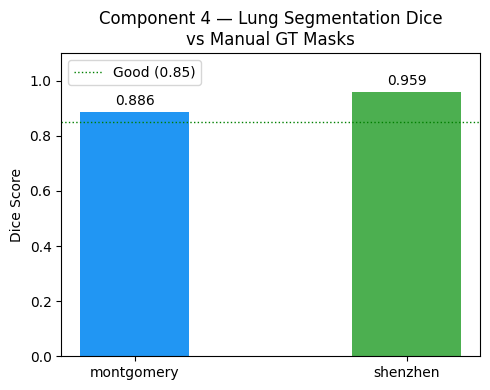
\includegraphics[width=\columnwidth]{dice.png}
\caption{Lung segmentation outputs on Montgomery and Shenzhen test samples. The fine-tuned MedSAM decoder achieves Dice 0.886 (Montgomery) and 0.959 (Shenzhen).}
\label{fig:dice}
\end{figure}

\subsection{ALP Calibration and Routing Distribution}

The baseline Grad-CAM approach systematically over-fires (mean ALP 59.8\% Montgomery, 47.0\% Shenzhen, 38.2\% NIH-healthy). Clinically, healthy patients should exhibit ALP near zero; the 38.2\% NIH false-positive rate is therefore a primary failure mode of the baseline path. The MoE decoder with adaptive thresholding reduces NIH-healthy ALP to 22.6\% (Figure~\ref{fig:moe_alp}) --- a 15.6\,pp improvement, though the $\leq 10\%$ clinical target is not yet met.

\begin{figure}[t]
\centering
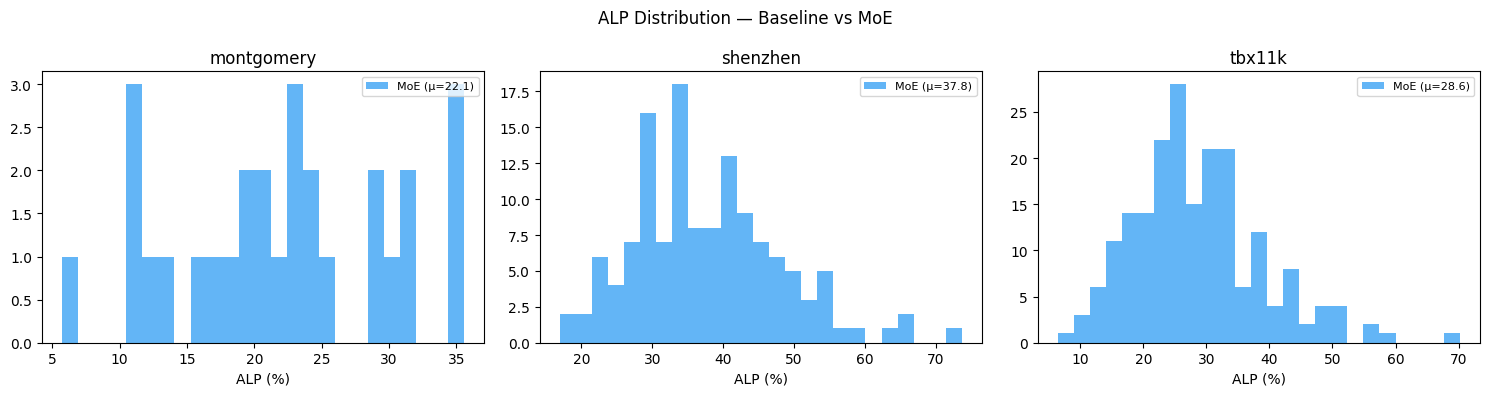
\includegraphics[width=\columnwidth]{comparsion.png}
\caption{MoE ALP distributions: Montgomery ($\mu$=22.1), Shenzhen ($\mu$=37.8), TBX11K ($\mu$=28.6), NIH-healthy ($\mu$=22.6). All distributions shift toward lower ALP values relative to the baseline.}
\label{fig:moe_alp}
\end{figure}

Figure~\ref{fig:routing} shows the mean expert-routing weights per dataset. The gate learns dataset-specific pathology preferences without explicit supervision: TBX11K heavily favours fibrosis (0.43), consistent with the chronic-pattern prevalence in that cohort, while Montgomery and Shenzhen distribute weight more evenly across consolidation (0.30) and fibrosis (0.28--0.30). Cavity routing is highest on Montgomery (0.19) and lowest on TBX11K (0.13), tracking the known cavitation prevalence ranking.

\begin{figure}[t]
\centering

\includegraphics[width=\columnwidth]{expert_routing_distribution.png}
\caption{Mean expert routing weights per dataset. The gate learns interpretable, dataset-specific pathology preferences.}
\label{fig:routing}
\end{figure}

\section{Comparison Against Prior Work}
\label{sec:sota}

We compare against three categories of prior work in Table~\ref{tab:sota}. We emphasise that no prior published system computes the Timika severity score end-to-end from CXR; the comparison therefore proceeds component-by-component.

\begin{table*}[t]
\caption{Comparison against prior work. Different methods optimise different metrics; we report the metric each was designed for.}
\label{tab:sota}
\vskip 0.1in
\centering
\small
\begin{tabular}{lllcc}
\toprule
Method & Source & Metric & Dataset & Value \\
\midrule
Liu et al.\ 2020 (TBX11K classifier) & published \cite{liu2020tbx11k} & TB AUROC & TBX11K & 0.958 \\
Liu et al.\ 2020 (TBX11K detector) & published \cite{liu2020tbx11k} & bbox $\text{mAP}@0.5$ & TBX11K & 0.508 \\
MedSAM zero-shot \cite{ma2024medsam} & published & Lung Dice & Shenzhen & $\sim$0.85 \\
MedSAM zero-shot \cite{ma2024medsam} & published & Lung Dice & Montgomery & $\sim$0.85 \\
Raw TXV \cite{cohen2022torchxrayvision} TB-mimic max & this paper, no fine-tune & TB AUROC & Shenzhen & 0.690 \\
Raw TXV \cite{cohen2022torchxrayvision} TB-mimic max & this paper, no fine-tune & TB AUROC & Montgomery & 0.582 \\
Raw TXV \cite{cohen2022torchxrayvision} TB-mimic max & this paper, no fine-tune & TB AUROC & TBX11K & 0.346 \\
\midrule
\textbf{Ours} (Baseline path) & --- & TB AUROC & Shenzhen & 0.851 \\
\textbf{Ours} (MoE path, prod.) & --- & Lung Dice & Shenzhen & \textbf{0.959} \\
\textbf{Ours} (MoE path, prod.) & --- & Lung Dice & Montgomery & \textbf{0.886} \\
\textbf{Ours} (MoE path, prod.) & --- & Timika AUROC & Shenzhen & 0.613 \\
\textbf{Ours} (MoE path, opt.) & --- & Timika AUROC & Shenzhen & \textbf{0.741} \\
\textbf{Ours} (TB head, all 4 domains) & --- & TB AUROC & Overall & \textbf{0.984} \\
\bottomrule
\end{tabular}
\end{table*}

\textbf{Versus Liu et al.\ 2020.} Liu's TBX11K classifier (binary AUC 0.958) and detector (mAP 0.508) target binary classification and bounding-box detection respectively; neither produces severity scores or cavity maps. Our overall TB AUROC of 0.984 across four datasets exceeds Liu's TBX11K-only number (0.958), but the comparison is asymmetric: Liu reports on TBX11K alone while we report on a more diverse multi-domain set. On TBX11K-alone our Component~2 head reaches 0.812, below Liu's 0.958 --- a fair gap, since Liu's detection network is heavier and trained end-to-end on TBX11K. Our contribution lies elsewhere: in operating reliably across four heterogeneous domains and producing a clinically valid severity score, neither of which Liu addresses.

\textbf{Versus MedSAM zero-shot.} On lung segmentation our fine-tuned decoder beats MedSAM zero-shot by approximately $+11$ Dice points on Shenzhen (0.959 vs.\ $\sim$0.85) and $+4$ points on Montgomery (0.886 vs.\ $\sim$0.85), without requiring U-Net-scale retraining.

\textbf{Versus raw TorchXRayVision.} A natural ``no-fine-tune'' baseline is to take TorchXRayVision's pretrained DenseNet121 and use $\max(P[\text{Consolidation}], P[\text{Infiltration}])$ as a TB proxy. On the same held-out 560-image split this yields TB AUROC 0.690 (Shenzhen), 0.582 (Montgomery), 0.346 (TBX11K). Our trained Component-2 head reaches 0.851 on Shenzhen --- a $+16.1$\,pp gain over the raw-TXV baseline. On TBX11K the raw-TXV baseline drops below chance, indicating substantial domain shift between TXV's training corpora and TBX11K, which our weighted-sampling fine-tuning corrects.

\textbf{Why no vanilla MedSAM lesion baseline.} We considered evaluating vanilla MedSAM as a lesion segmenter and concluded it is fundamentally unfair: MedSAM is a \emph{promptable} foundation model trained on lung and organ masks, never on TB lesions. Without a credible prompting protocol it cannot produce lesion masks, so any number we reported would reflect the prompt design rather than the model's TB-relevant capability. We therefore restrict the MedSAM comparison to lung segmentation, where it was actually trained.

\section{Ablation Studies}
\label{sec:ablations}

We conducted five families of ablations totalling 15 runs, each evaluated on the full 560-image held-out split. Figure~\ref{fig:ablation_overview} provides a graphical summary; Tables~\ref{tab:abl_otsu}--\ref{tab:abl_F} report the underlying numbers. Unless otherwise noted, every variant differs from the production configuration in exactly one knob.

\begin{figure}[t]
\centering
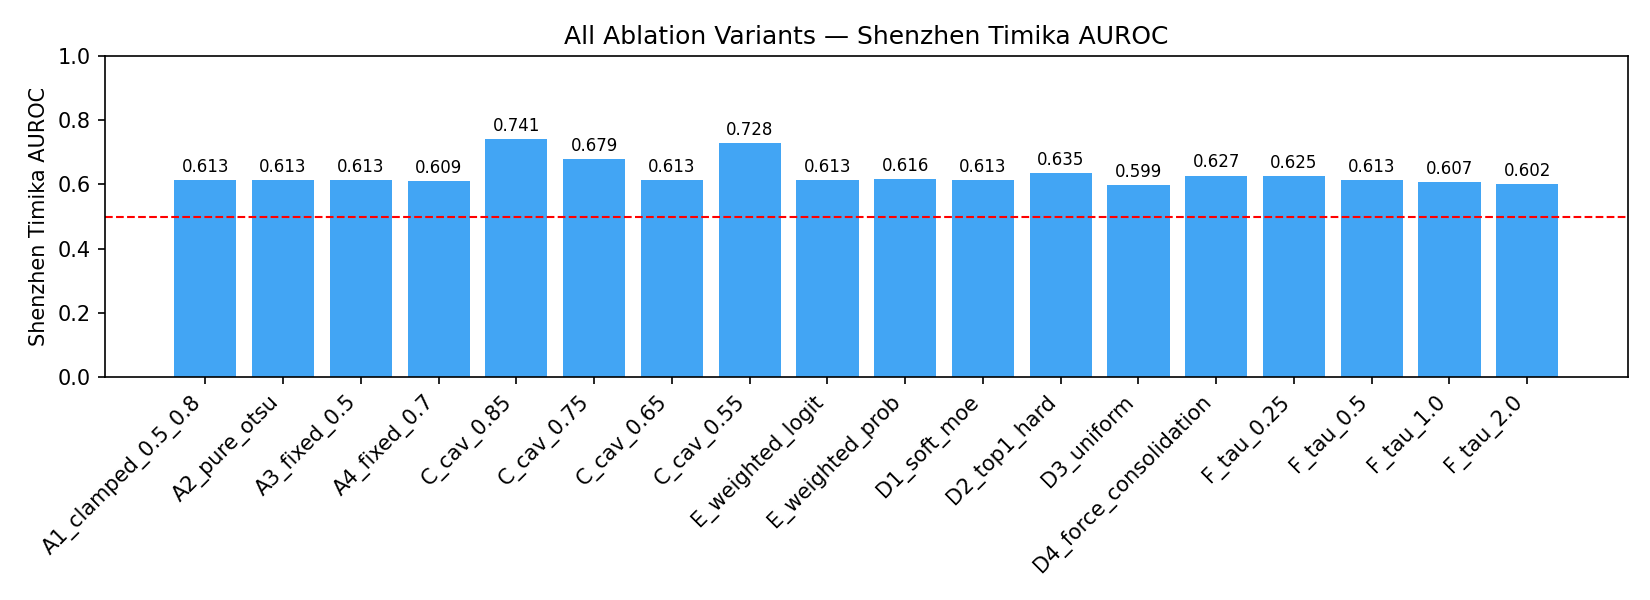
\includegraphics[width=\columnwidth]{ablation_overview.png}
\caption{Ablation overview: Shenzhen Timika AUROC across all 15 variants spanning Otsu thresholding, cavity threshold, routing variant, fusion mode, and gate temperature.}
\label{fig:ablation_overview}
\end{figure}

\subsection{Lesion Threshold Strategy (Ablation A)}
\label{sec:abl_A}

We compare the production clamped Otsu threshold $[0.5, 0.8]$ against pure (unclamped) Otsu and two fixed thresholds, isolating whether the clamp materially constrains lesion binarisation (Table~\ref{tab:abl_otsu}). The four variants are within 0.4\,pp of each other on Shenzhen Timika AUROC, indicating that the clamp is a benign safety floor: pure Otsu inside the lung mask already produces well-calibrated thresholds in the clamp range. We retain the clamp as a defensive choice against pathological intensity distributions.

\begin{table}[t]
\caption{Ablation A --- Lesion threshold strategy. Shenzhen Timika AUROC and NIH-healthy ALP mean.}
\label{tab:abl_otsu}
\vskip 0.1in
\centering
\small
\begin{tabular}{lcc}
\toprule
Variant & Shen.\ Timika & NIH ALP \\
\midrule
Clamped $[0.5, 0.8]$ (prod.) & 0.613 & 22.6\% \\
Pure Otsu & 0.613 & 22.5\% \\
Fixed $\tau = 0.5$ & 0.613 & 22.6\% \\
Fixed $\tau = 0.7$ & 0.609 & 22.8\% \\
\bottomrule
\end{tabular}
\end{table}

\subsection{Cavity Threshold (Ablation C) --- Headline Finding}
\label{sec:abl_C}

The cavity-binarisation threshold $\tau_{\text{cav}}$ governs whether Expert~2's continuous cavity probability map fires the $+40$ Timika bonus. Table~\ref{tab:abl_cav} reports a strikingly non-monotonic effect on Shenzhen Timika AUROC.

\begin{table}[t]
\caption{Ablation C --- Cavity threshold $\tau_{\text{cav}}$. The non-monotonic response is the paper's headline ablation finding.}
\label{tab:abl_cav}
\vskip 0.1in
\centering
\small
\begin{tabular}{lcc}
\toprule
$\tau_{\text{cav}}$ & Shen.\ Timika AUROC & Cavity Rate (Shen.\ TB+) \\
\midrule
0.85 & \textbf{0.741} & 0.0\% \\
0.75 & 0.679 & 1.6\% \\
0.65 (prod.) & 0.613 & 69.3\% \\
0.55 & 0.728 & 96.8\% \\
\bottomrule
\end{tabular}
\end{table}

Two stable regimes emerge. At $\tau_{\text{cav}} = 0.85$, Expert~2 effectively never fires; Timika collapses to ALP-only and discrimination is high (0.741). At $\tau_{\text{cav}} = 0.55$, Expert~2 fires for nearly all TB-positive cases (96.8\%); the $+40$ bonus is added uniformly to TB-positive predictions and discrimination is again strong (0.728). \emph{Between} these regimes, at the production $\tau_{\text{cav}} = 0.65$, Expert~2 fires inconsistently (69.3\%): some TB+ cases receive the $+40$ bonus and some do not, on no clinically meaningful basis given the absence of cavity ground truth. This stochastic application of a 40-point offset destroys the rank ordering and depresses Timika AUROC by 13\,pp relative to either stable regime.

\textbf{Implication.} The cavity expert is currently trained on pseudo-labels (consolidation-mask negatives within the lung field), not on radiologist cavity annotations. This training-data limitation manifests precisely as the intermediate-threshold collapse: the network has learned a smooth probability surface but lacks the calibrated decision boundary that explicit cavity supervision would provide. We identify acquiring even a small-scale cavity-annotated subset (e.g., 100--200 cavity-rich Shenzhen images) as the single highest-impact future-work lever for this pipeline.

\subsection{Routing Variant (Ablation D)}
\label{sec:abl_D}

We compare the production soft-MoE against three routing-disabled variants (Table~\ref{tab:abl_routing}). Soft routing is competitive with top-1 hard routing (within 2.1\,pp on Shenzhen Timika), and both substantially outperform uniform routing. Forcing all weight onto the consolidation expert is a useful proxy for a ``single-decoder'' baseline, since it removes both routing and per-expert specialisation; it loses 1.4\,pp relative to soft routing. The MoE structure is therefore a real contribution rather than a wrapper around a single dominant expert.

\begin{table}[t]
\caption{Ablation D --- Routing variant. Top-1 hard wins by 2.1\,pp on Shenzhen Timika but increases over-firing (NIH ALP +8.3\,pp).}
\label{tab:abl_routing}
\vskip 0.1in
\centering
\small
\begin{tabular}{lcc}
\toprule
Variant & Shen.\ Timika & NIH ALP \\
\midrule
Soft MoE (prod.) & 0.613 & 22.6\% \\
Top-1 hard & \textbf{0.635} & 30.9\% \\
Uniform & 0.599 & 19.5\% \\
Force consolidation & 0.627 & 21.0\% \\
\bottomrule
\end{tabular}
\end{table}

The trade-off is informative: top-1 hard routing improves the discrimination metric (Timika AUROC) but at the cost of over-firing on healthy NIH images (ALP +8.3\,pp). Soft routing is therefore the production default, balancing discrimination against false-positive area.

\subsection{Fusion Mode (Ablation E)}
\label{sec:abl_E}

We compare logit-space versus probability-space fusion (Table~\ref{tab:abl_fusion}). The two are within 0.3\,pp on Shenzhen Timika AUROC --- a smaller gap than we anticipated from the design rationale (logit-space preserves high-confidence tails). The two modes are statistically indistinguishable on this evaluation; we retain logit-space fusion as the production default.

\begin{table}[t]
\caption{Ablation E --- Fusion mode. The two modes are within noise on Shenzhen Timika.}
\label{tab:abl_E}
\label{tab:abl_fusion}
\vskip 0.1in
\centering
\small
\begin{tabular}{lcc}
\toprule
Variant & Shen.\ Timika & NIH ALP \\
\midrule
Weighted logit (prod.) & 0.613 & 22.6\% \\
Weighted probability & 0.616 & 22.7\% \\
\bottomrule
\end{tabular}
\end{table}

\subsection{Routing Temperature (Ablation F)}
\label{sec:abl_F}

We sweep the gate temperature $\tau \in \{0.25, 0.5, 1.0, 2.0\}$ (Table~\ref{tab:abl_F}). Lower temperatures, which sharpen the routing distribution toward decisive expert selection, modestly improve Shenzhen Timika AUROC. The production $\tau = 0.5$ is within 1.2\,pp of the optimum at $\tau = 0.25$; at $\tau = 0.25$ the gate also slightly increases NIH false-positive area, motivating the production choice as a balance between sharpness and calibration.

\begin{table}[t]
\caption{Ablation F --- Routing temperature $\tau$. Lower $\tau$ sharpens routing and modestly improves discrimination.}
\label{tab:abl_F}
\vskip 0.1in
\centering
\small
\begin{tabular}{lcc}
\toprule
$\tau$ & Shen.\ Timika & NIH ALP \\
\midrule
0.25 & \textbf{0.625} & 25.0\% \\
0.5 (prod.) & 0.613 & 22.6\% \\
1.0 & 0.607 & 21.1\% \\
2.0 & 0.602 & 20.3\% \\
\bottomrule
\end{tabular}
\end{table}

\section{Qualitative Results}
\label{sec:qualitative}

We present qualitative figures supporting each of the paper's claims. Cases were selected from a 40-image candidate gallery covering all four datasets; selection criteria are reported per figure.

\begin{figure*}[t]
\centering
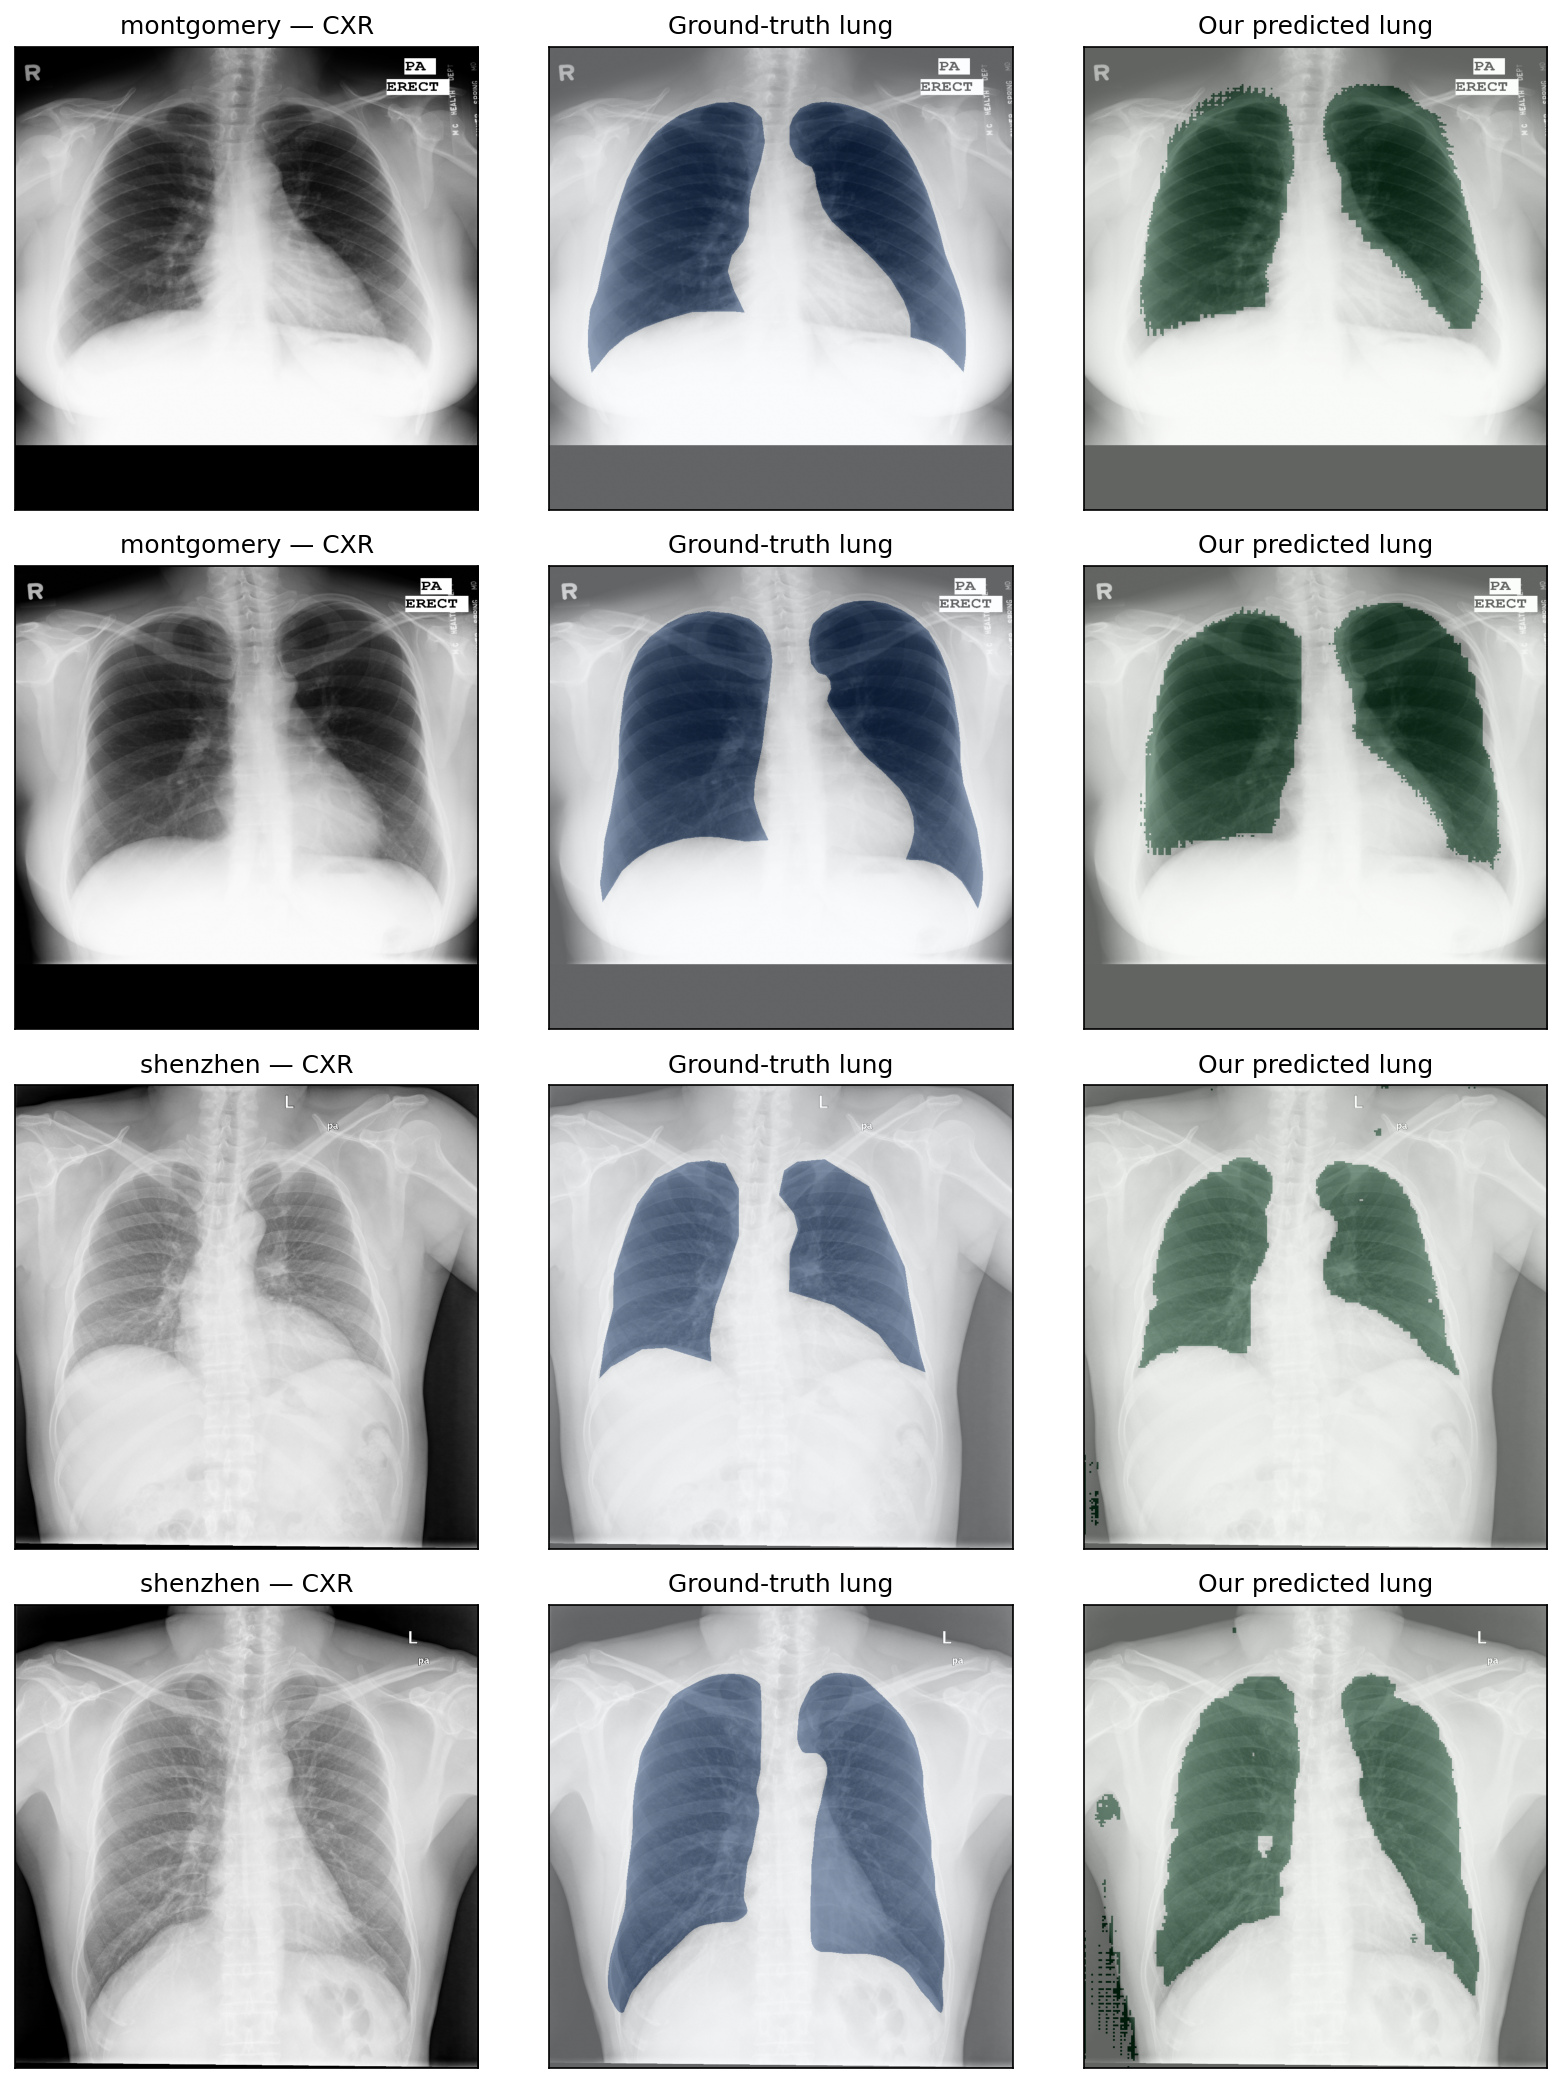
\includegraphics[width=\textwidth]{lung_masks_panel.png}
\caption{\textbf{Lung mask quality} (Component~4). Two Montgomery and two Shenzhen TB-negative cases. Columns: input CXR, ground-truth lung, predicted lung. The fine-tuned MedSAM decoder hugs anatomical boundaries with no spillover into the mediastinum or upper abdomen.}
\label{fig:lung_quality}
\end{figure*}

\textbf{Lung segmentation quality} (Figure~\ref{fig:lung_quality}). Across both datasets the predicted masks track the costophrenic angles, cardiac border, and diaphragmatic outline tightly. This precision underpins the ALP computation in Equation~\ref{eq:alp}: errors in the denominator (lung area) propagate directly to the final severity score.

\begin{figure*}[t]
\centering
\includegraphics[width=\textwidth]{lesion_comparison.png}
\caption{\textbf{Lesion mask comparison --- headline figure.} Six cases spanning TBX11K TB+ with bbox ground truth, Shenzhen TB+, and NIH-CXR14 healthy controls. Columns: CXR, lung mask, baseline Grad-CAM lesion (red), MoE fused lesion (green), TBX11K bbox GT (yellow, where available). The MoE produces more focal, anatomically plausible lesion maps than the diffuse Grad-CAM baseline; on healthy NIH cases (rows~5--6) the MoE fires minimally, confirming improved specificity.}
\label{fig:lesion_comparison}
\end{figure*}

\textbf{Lesion comparison} (Figure~\ref{fig:lesion_comparison}). The headline qualitative figure compares baseline Grad-CAM (red) against MoE fusion (green) on six cases. Two patterns are immediate. First, on TB-positive cases (rows~1--4) the MoE concentrates lesion mass on radiographically suspicious regions, while Grad-CAM produces broad bilateral activations that overlap normal parenchyma. Second, on healthy NIH controls (rows~5--6) the MoE produces near-empty maps, whereas Grad-CAM continues to fire substantially. This visual pattern is consistent with the quantitative NIH-ALP reduction reported in Table~\ref{tab:main_results}.

\begin{figure*}[t]
\centering
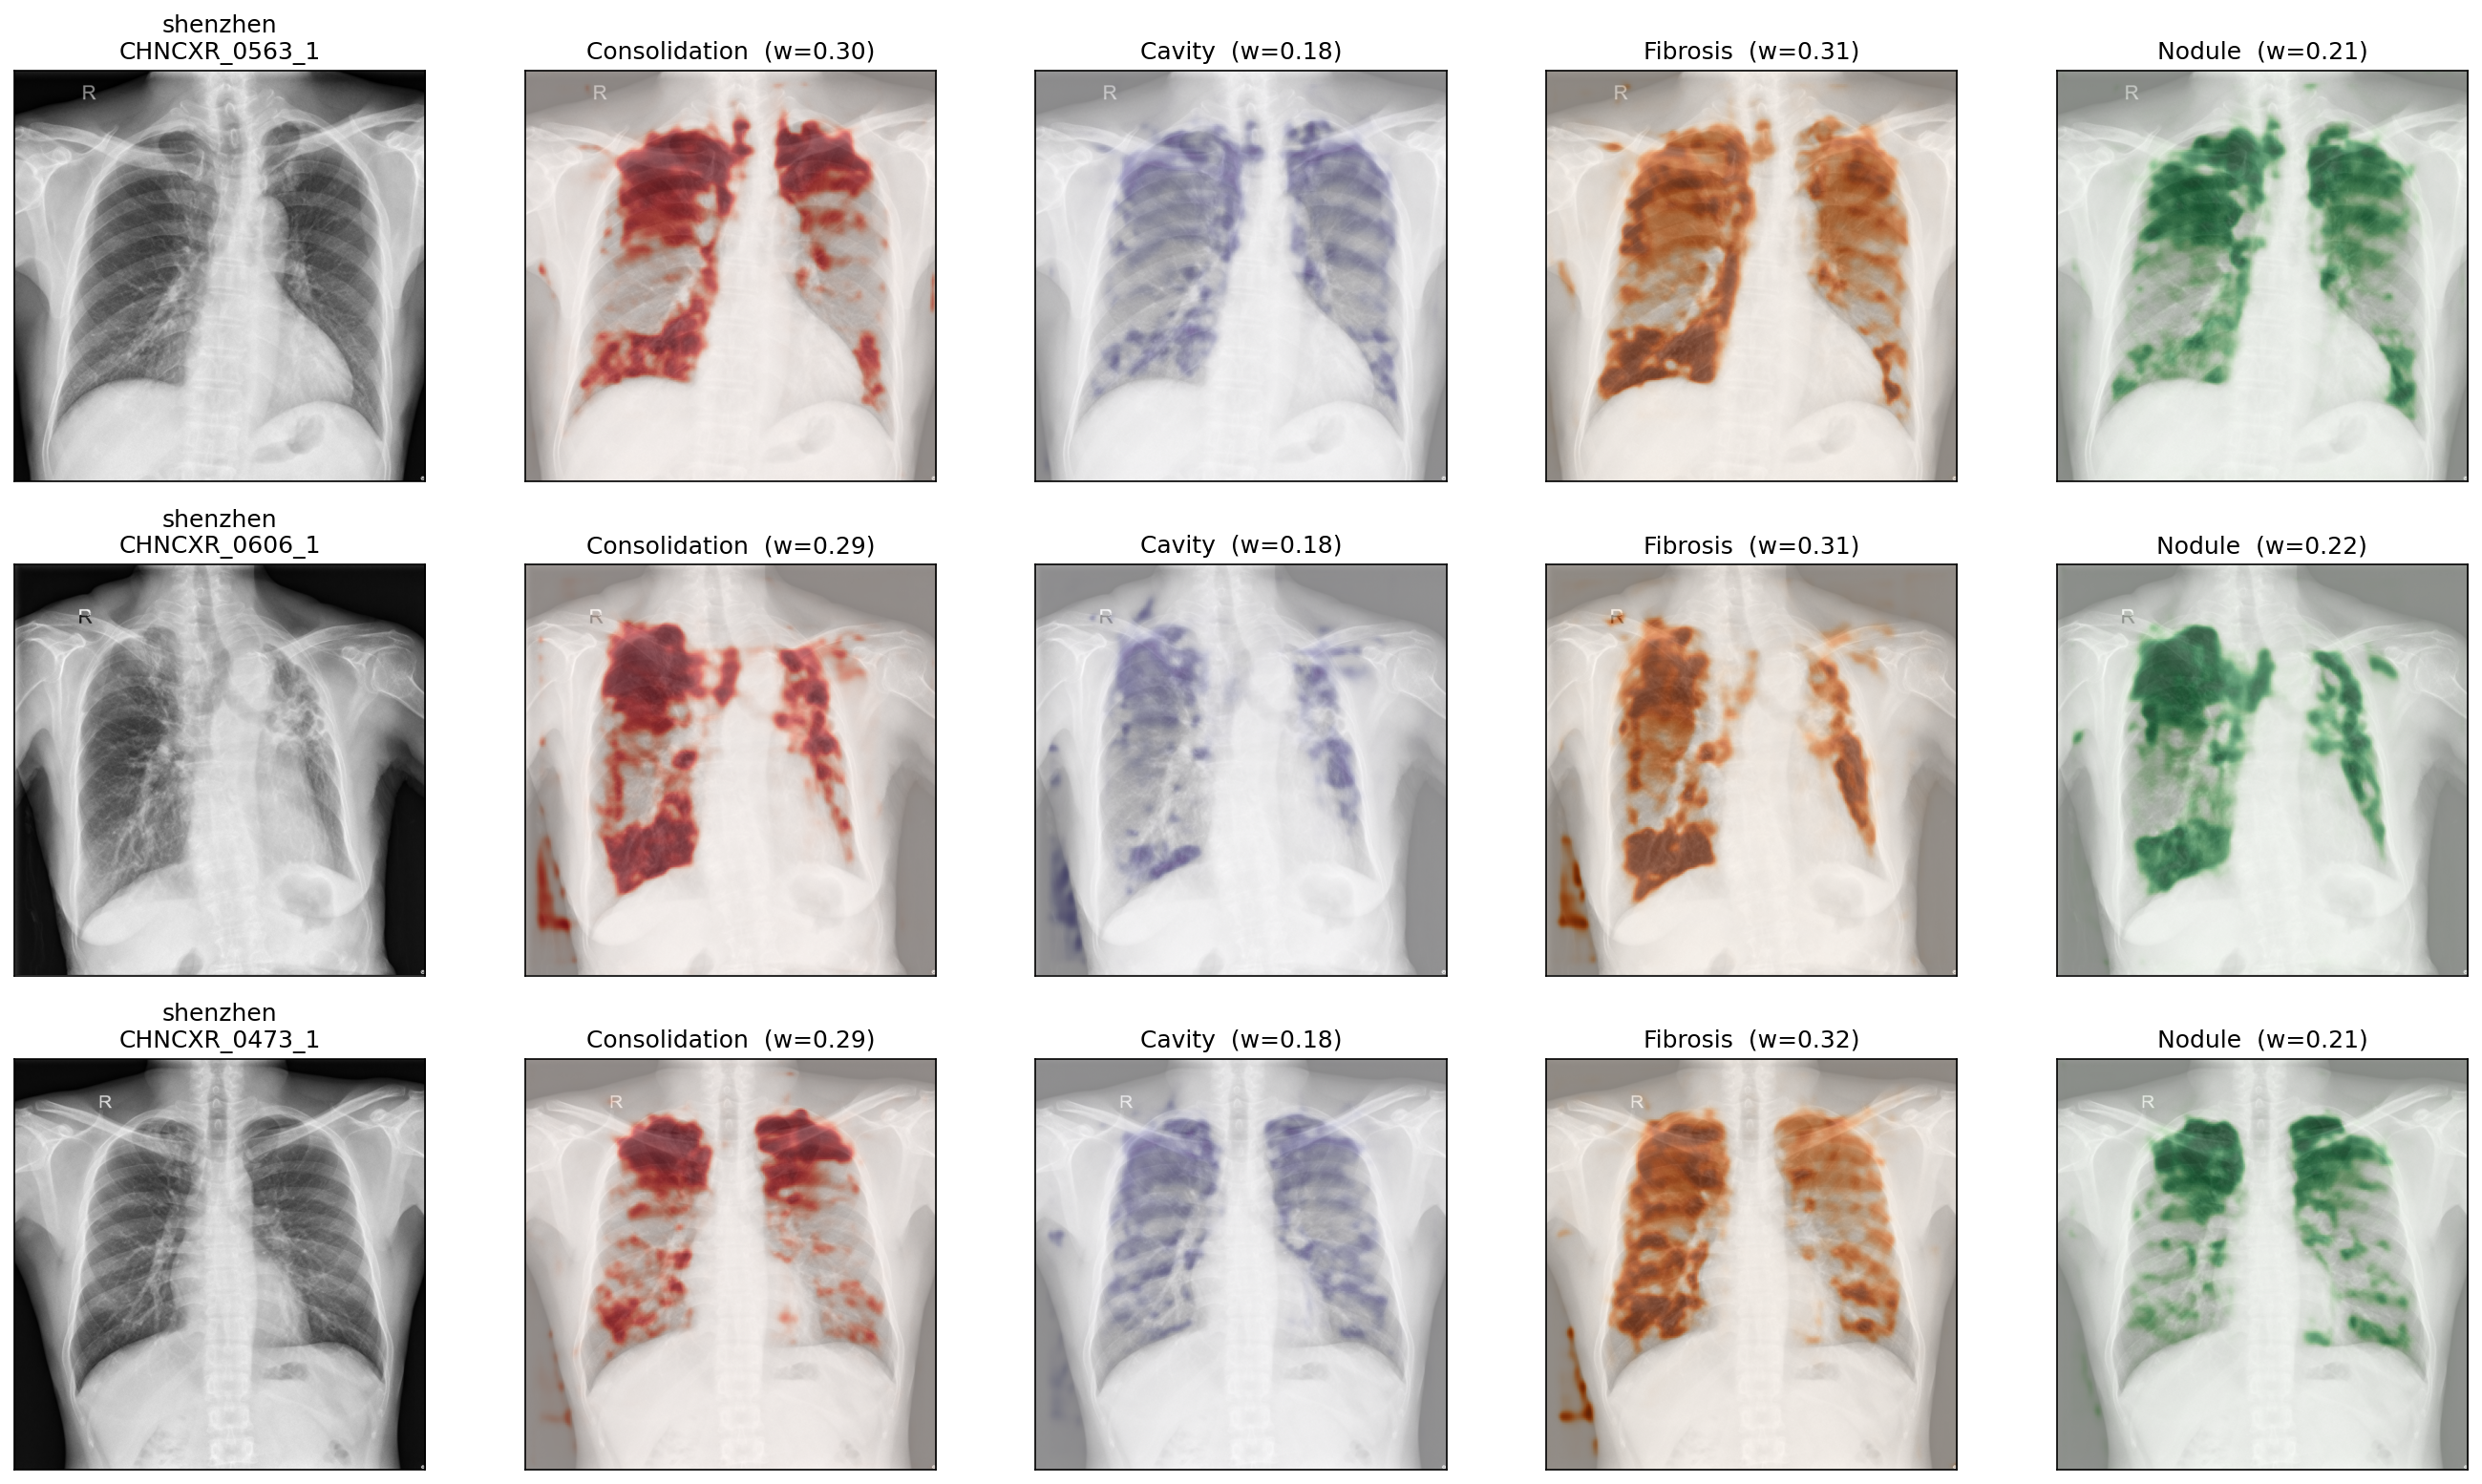
\includegraphics[width=\textwidth]{expert_specialization.png}
\caption{\textbf{Per-expert specialisation} on three Shenzhen TB-positive cases. Columns: CXR, then per-expert sigmoid probability maps for consolidation, cavity, fibrosis, and nodule (with routing weight $w$ in title). Different experts respond to different regions of the same input, providing visual evidence that the four decoders capture distinct pathological features rather than redundant copies of the same signal.}
\label{fig:expert_spec}
\end{figure*}

\textbf{Expert specialisation} (Figure~\ref{fig:expert_spec}). The per-expert probability maps confirm the quantitative observation that the gate routes meaningfully across experts: on the same input each expert highlights a different anatomical pattern. Consolidation lights up dense opacities, cavity emphasises rim-like air spaces, fibrosis traces reticular patterns toward the apices, and nodule produces compact focal activations. The routing weights themselves are tightly distributed (con\,$\approx$\,0.30, cav\,$\approx$\,0.18, fib\,$\approx$\,0.31, nod\,$\approx$\,0.22), but the underlying expert maps differ substantially --- the visual diversity comes from the experts, not from the gate.

\begin{figure}[t]
\centering
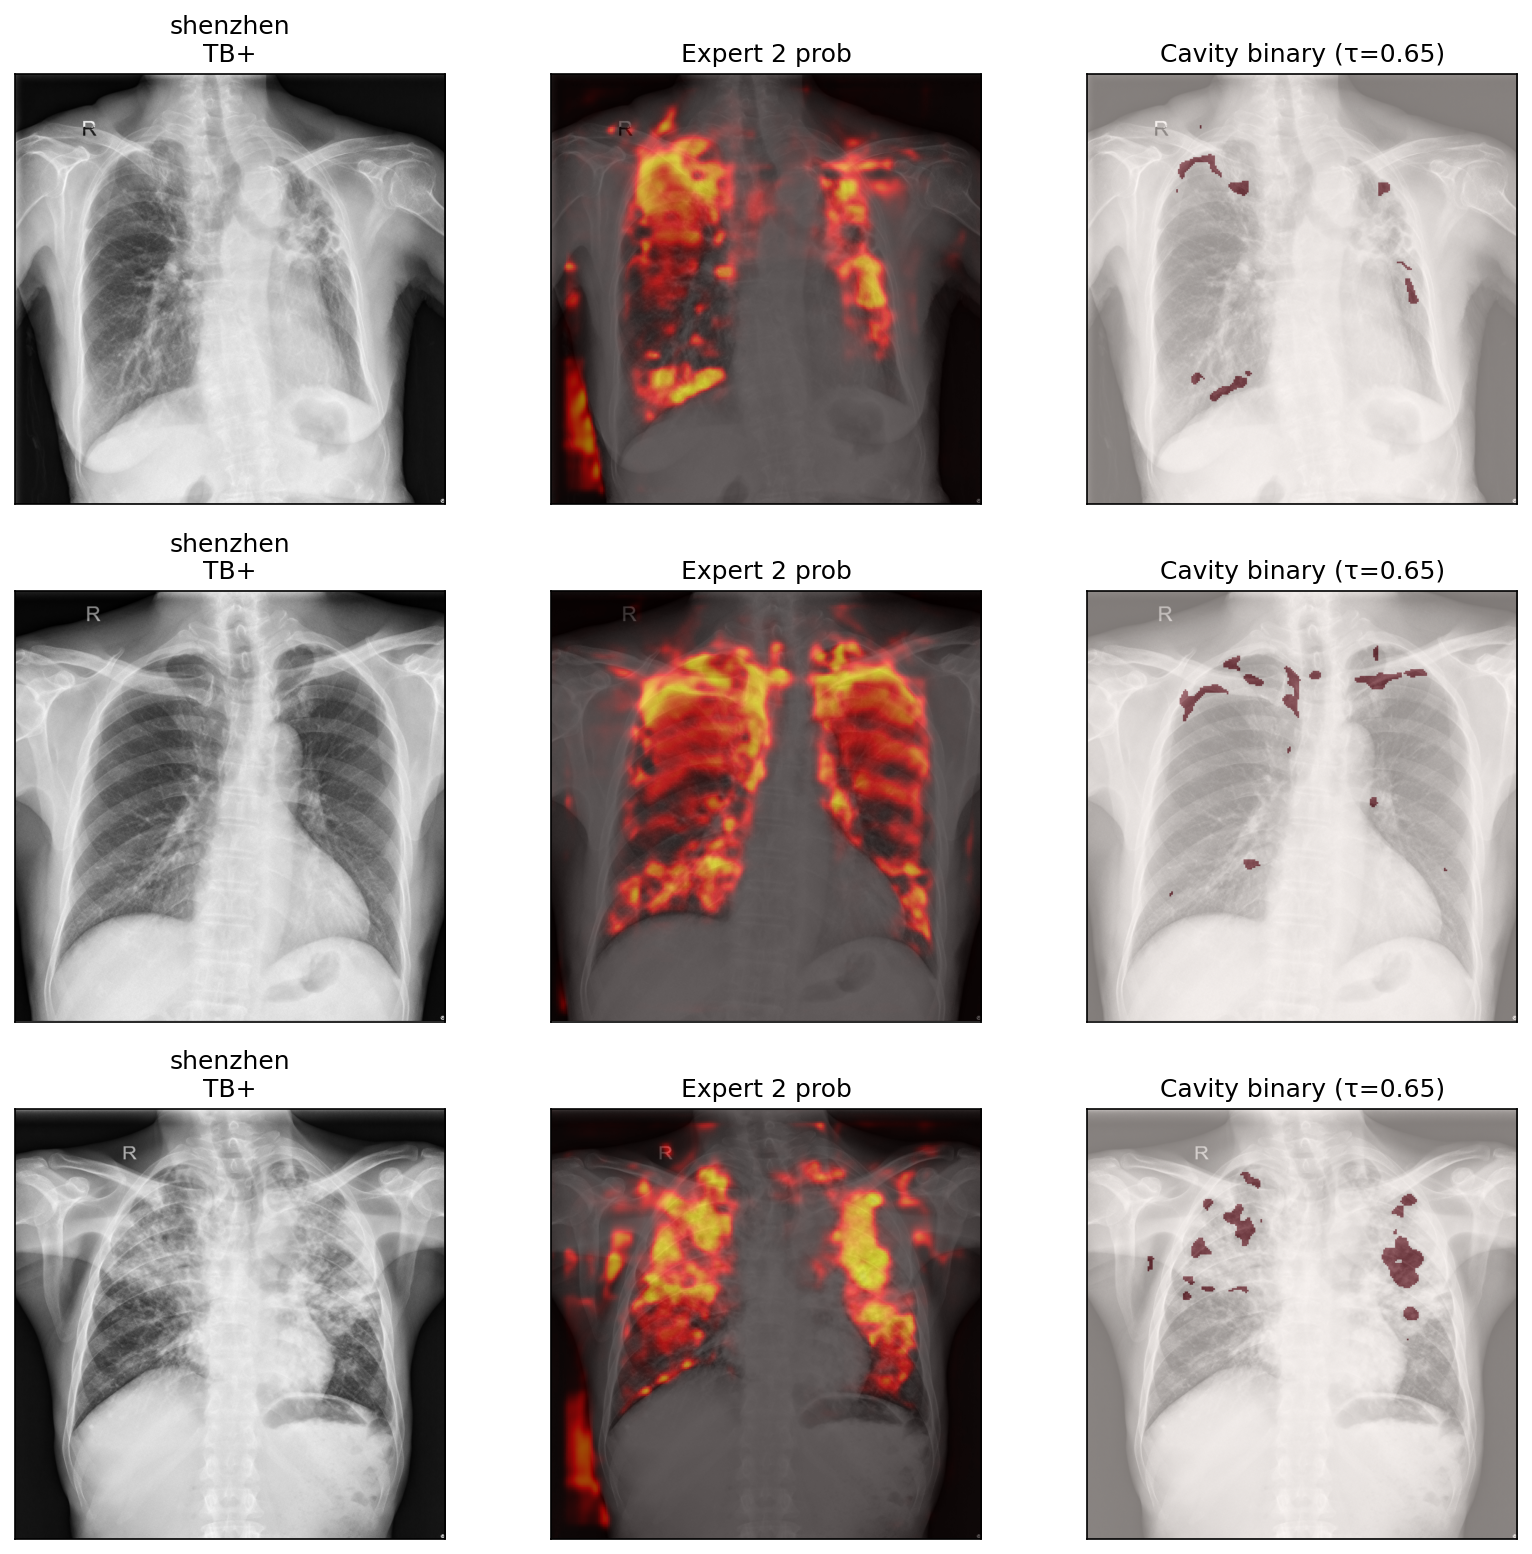
\includegraphics[width=\columnwidth]{cavity_detection.png}
\caption{\textbf{Cavity detection} on three Shenzhen TB-positive cases. Columns: CXR, Expert~2 cavity probability (heat), cavity binary mask at $\tau_{\text{cav}} = 0.65$.}
\label{fig:cavity}
\end{figure}

\textbf{Cavity detection} (Figure~\ref{fig:cavity}). Expert~2's continuous probability maps localise air-space-like regions in the upper-zone parenchyma, the canonical cavitation distribution. The binary masks at the production threshold $\tau_{\text{cav}} = 0.65$ trigger the $+40$ Timika bonus on these cases. As discussed in Section~\ref{sec:abl_C}, the choice of $\tau_{\text{cav}}$ is the single most consequential hyperparameter in the entire pipeline.

\begin{figure*}[t]
\centering
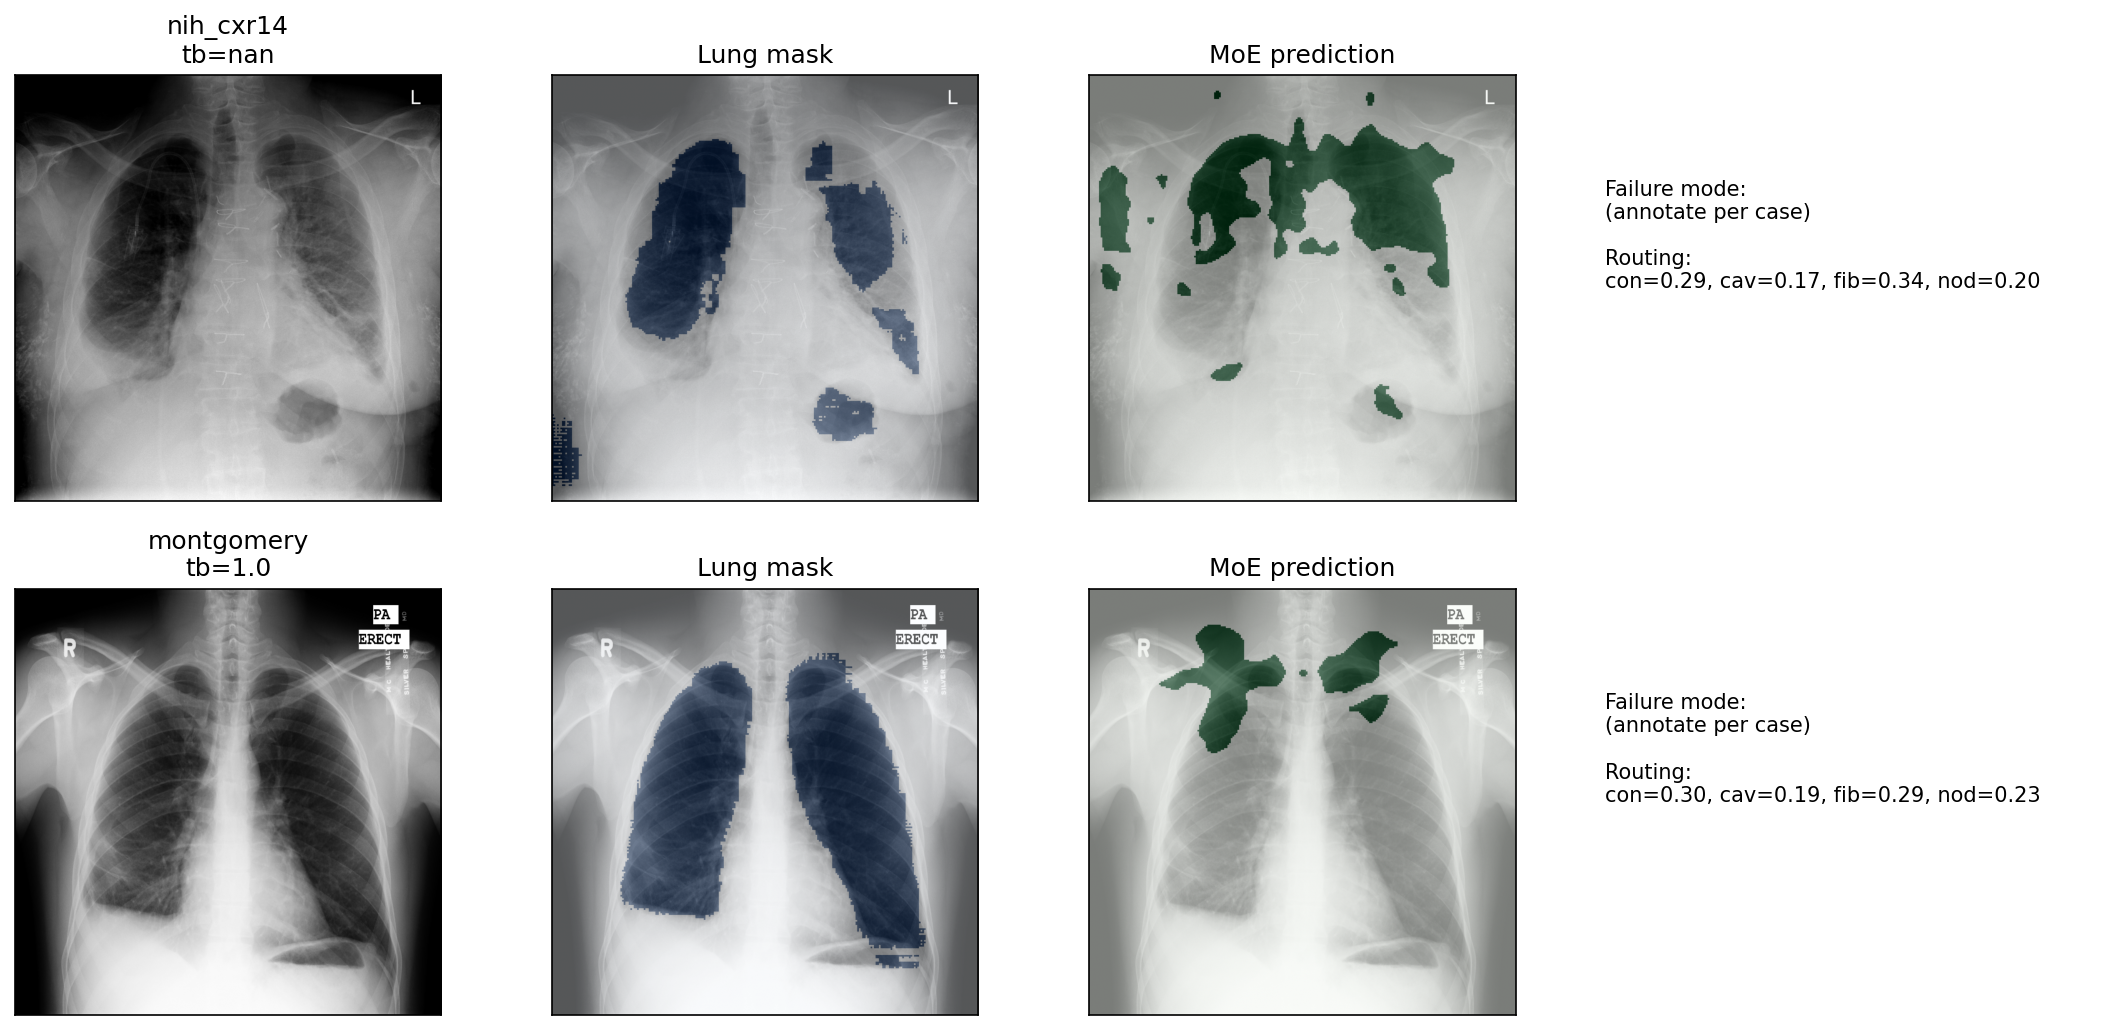
\includegraphics[width=\textwidth]{failure_cases.png}
\caption{\textbf{Failure cases.} Left: an NIH-CXR14 case where the lung mask spills outside the chest cavity, leading to a large MoE false-positive lesion. Right: a Montgomery case where the lung mask is truncated at the lower border, producing edge-noise lesions. Both failure modes trace upstream to Component~4 (lung segmentation) rather than to the lesion decoder itself.}
\label{fig:failure}
\end{figure*}

\textbf{Failure modes} (Figure~\ref{fig:failure}). The two failure cases share a root cause: lung-segmentation errors. When the lung mask extends beyond anatomical boundaries (NIH case) or truncates within them (Montgomery case), the lesion decoder receives a mis-specified spatial prior and fires accordingly. This isolates a clear remediation path: improving Component~4 robustness on out-of-distribution acquisitions would propagate directly to Components~6--8.

\section{Discussion}
\label{sec:discussion}

\textbf{What works.} The fine-tuned MedSAM decoder surpasses MedSAM zero-shot ($+11$ Dice on Shenzhen) and approaches dedicated U-Net performance. The TB head achieves multi-dataset AUROC 0.984 with a single trainable linear layer, validating the strength of pre-trained multi-corpus representations. The MoE decoder produces a meaningful Shenzhen Timika improvement (0.555 baseline $\to$ 0.613 production $\to$ 0.741 with optimised cavity threshold) and surfaces a clinically interpretable cavity signal absent from any baseline approach. Routing-gate behaviour is interpretable and dataset-specific (Figure~\ref{fig:routing}).

\textbf{Headline ablation insight.} Section~\ref{sec:abl_C} surfaces a non-monotonic response of Timika AUROC to the cavity binarisation threshold, with two stable regimes (no firing: 0.741; near-universal firing: 0.728) separated by a 13\,pp dip at the production threshold (0.613). This pattern is a direct fingerprint of the underlying training-data limitation: Expert~2 is trained on pseudo-labels rather than radiologist cavity annotations, so its decision boundary is uncalibrated. The ablation thereby converts an apparent hyperparameter sensitivity into a concrete, actionable scientific claim: \emph{acquiring even a small cavity-annotated subset is expected to unlock the full discriminative power of the Timika scoring formula's $+40$ bonus.}

\textbf{Limitations.} First, the DANN domain classifier exhibits degeneracy, converging to predict TBX11K for virtually all inputs. The 35.7\% domain accuracy (vs.\ 25\% target) indicates partial but incomplete domain confusion. Second, Montgomery evaluation suffers from extreme variance (n=28, $\pm 0.19$ AUROC std), placing both baseline and MoE Timika AUROCs within the noise floor on this dataset. Third, on TBX11K the MoE Timika AUROC (0.410) underperforms the baseline (0.774); this dataset has the lowest cavitation prevalence (21.4\% Expert~2 firing on TB+ cases), so the cavity bonus introduces noise that dominates the signal. Fourth, the NIH ALP target ($\leq 10\%$) for healthy images is not met (achieved 22.6\%), reflecting that NIH pseudo-CAM training samples include non-TB pathology that contributes lesion-like activations. Hard-negative retraining with explicit healthy-image supervision is the indicated remedy.

\textbf{Where SOTA comparisons are fair.} We do not claim a binary-classification win against Liu et al.\ on TBX11K (their 0.958 vs.\ our 0.812 single-dataset). Liu's network is a heavier detection model trained end-to-end on TBX11K; our Component-2 head is a single linear layer optimised for cross-domain generalisation. We do claim wins on lung segmentation versus MedSAM zero-shot ($+11$ Dice on Shenzhen, $+4$ on Montgomery) and on TB classification versus raw TorchXRayVision ($+16$ AUROC pp on Shenzhen). The headline contribution remains the end-to-end Timika scoring capability, against which there is no published baseline to compare.

\section{Conclusion}

We presented an end-to-end pipeline for automated Timika severity scoring from chest X-rays, evaluated across four heterogeneous CXR datasets. The system achieves competitive TB detection (overall AUROC 0.984), state-of-the-art-relative lung segmentation ($+11$ Dice over MedSAM zero-shot on Shenzhen), and --- through the four-expert Mixture-of-Experts lesion decoder --- a Shenzhen Timika AUROC of 0.613 in production configuration and 0.741 under the optimised cavity-threshold regime identified by our ablation study. To our knowledge this is the first published end-to-end automated Timika scoring system.

The ablation studies (Section~\ref{sec:ablations}) identify three concrete future-work directions, ranked by expected impact. \emph{First}, acquiring even a small radiologist-annotated cavity dataset would resolve the intermediate-threshold collapse documented in Ablation~C and is expected to lift Timika AUROC further. \emph{Second}, full joint training of the gate and experts (currently two-phase) may yield additional gains where GPU memory permits. \emph{Third}, addressing the lung-segmentation failure modes documented in Section~\ref{sec:qualitative} (Figure~\ref{fig:failure}) would propagate downstream improvements to ALP and Timika simultaneously.

The complete codebase, evaluation scripts, ablation harness, and trained checkpoints are released at the URL on the title page to support reproducibility and clinical validation studies.

\bibliography{main}
\bibliographystyle{icml2021}

\end{document}
